\chapter{Notations, Assumptions and Datasets}
\label{ch:Notations_Data}
\noindent{\textbf{\huge T}}his chapter introduces the notations and definitions used throughout the thesis. The methods presented in later chapters use the same notations as given here. We also state the common premises about datasets assumed by these methods. Towards the end of this chapter, we list the details of datasets used for experiments.



\section{Terminologies and Notations}
\label{sec:Notations}
\hspace{0.8cm}We use lowercase letters to denote a constant (e.g.- $n$, $n_{ij}$) and boldface lowercase letters for vectors (e.g.- $\textbf{x}_{ijk}$). A boldface capital letter (e.g.- $\textbf{S}_{jr}$) denotes a matrix, and a set is represented using calligraphic capital letter (e.g.- $\mathcal{X}$). The notations used in this thesis are listed in Table \ref{tab:Notations}.

As the methods presented in this thesis use either 1D or 2D data samples, the representation varies according to the dimensionality of data. This difference is presented here explicitly. However, at the subsequent mentions of the data samples in this chapter, only the 1D notations are used. Let us denote a multi-view dataset as $\mathcal{X}$. If it is a 1D dataset, it is defined as

\begin{center}
$\mathcal{X} = \left \{ \textbf{x}_{ijk} | i=1,\cdots,c; \;\; j=1,\cdots,v; \;\; k=1,\cdots,n_{ij} \right \}$
\end{center}

Here, each vector $\textbf{x}_{ijk}$ is the $k^{th}$ data sample from $j^{th}$ view of $i^{th}$ class and $n_{ij}$ is the number of data samples in $j^{th}$ view of $i^{th}$ class.

If $\mathcal{X}$ is a 2D dataset, each of its $k^{th}$ data sample from $i^{th}$ class of $j^{th}$ view is denoted as $\textbf{X}_{ijk}$. The dataset is defined as

\begin{center}
$\mathcal{X} = \left \{ \textbf{X}_{ijk} | i=1,\cdots,c; \;\; j=1,\cdots,v; \;\; k=1,\cdots,n_{ij} \right \}$
\end{center}

We denote the number of classes with $c$ and the number of views with $v$. The size of each data sample is $p_j \times q$. The value of $p_j$ may vary across the views, but it is the same for all data samples within a view. The value of $q$ is constant for all the data samples across all the views. For 1D datasets $q=1$.

Every data sample from the original space is projected into a common discriminant subspace using the projection matrix $\textbf{W} = \left[ \textbf{W}_1^T \textbf{W}_2^T \cdots \textbf{W}_v^T \right]^T $, where each $\textbf{W}_j$ is a $d \times p_j$ matrix that is used to project $j$th view. The data samples thus projected are denoted as

\begin{center}
$\mathcal{Y} = \left \{ \textbf{y}_{ijk} = \textbf{W}_j^T \textbf{x}_{ijk} | i=1,\cdots,c; j=1,\cdots,v; k=1,\cdots,n_{ij} \right \}$
\end{center}


\begin{table}[t]
	\centering
	\caption{Table shows how the entities are denoted with different notations for existing dataset ($\mathcal{X}$), added/deleted subset ($\bar{\mathcal{X}}$) and the updated dataset after addition/deletion ($\mathcal{X}'$).}
	\label{tab:Notations}
		\begin{tabular}{l c c c} \toprule
		Description & Existing & Added/Deleted & Updated \\
		\toprule
		Data sample of 1D dataset & $\textbf{x}_{ijk}$ & $\bar{\textbf{x}}_{ijk}$ & $\textbf{x}_{ijk}'$ \\[0.2cm]
		Data sample of 2D dataset & $\textbf{X}_{ijk}$ & $\bar{\textbf{X}}_{ijk}$ & $\textbf{X}_{ijk}'$ \\[0.2cm]
		Size of 1D data samples & $p_j \times 1$ & - & - \\[0.2cm]
		Size of 2D data samples & $p_j \times q$ & - & - \\[0.2cm]
		No. of classes & $c$ & $\bar{c}$ & $c'$ \\[0.2cm]
		Set of classes & $\mathcal{C}$ & $\bar{\mathcal{C}}$ & $\mathcal{C}'$ \\[0.2cm]
		No. of views & $v$ & $\bar{v}$ & $v'$ \\[0.2cm]
		Set of views & $\mathcal{V}$ & $\bar{\mathcal{V}}$ & $\mathcal{V}'$ \\[0.2cm]
		No. of data samples per class per view & $n_{ij}$ & $\bar{n}_{ij}$ & $n_{ij}'$ \\[0.2cm]
		No. of data samples per class & $n_{i}$ & $\bar{n}_{i}$ & $n_{i}'$ \\[0.2cm]
		No. of total data samples & $n$ & $\bar{n}$ & $n'$ \\[0.2cm]
		Mean per class per view of 1D dataset & $\textbf{m}_{ij}^{(\textbf{x})}$ & $\bar{\textbf{m}}_{ij}^{(\textbf{x})}$ & ${\textbf{m}_{ij}'}^{(\textbf{x})}$ \\[0.2cm]
		Class mean of 1D dataset & $\textbf{m}_{i}$ & $\bar{\textbf{m}}_{i}$ & $\textbf{m}_{i}'$ \\[0.2cm]
		Total mean of 1D dataset & $\textbf{m}$ & $\bar{\textbf{m}}$ & $\textbf{m}'$ \\[0.2cm]
		Mean per class per view of 2D dataset & $\textbf{M}_{ij}^{(\textbf{x})}$ & $\bar{\textbf{M}}_{ij}^{(\textbf{x})}$ & ${\textbf{M}_{ij}'}^{(\textbf{x})}$ \\[0.2cm]
		Class mean of 2D dataset & $\textbf{M}_{i}$ & $\bar{\textbf{M}}_{i}$ & $\textbf{M}_{i}'$ \\[0.2cm]
		Total mean of 2D dataset & $\textbf{M}$ & $\bar{\textbf{M}}$ & $\textbf{M}'$ \\[0.2cm]
		Within-class scatter in projected space & $\textbf{S}_W$ & - & $\textbf{S}_W'$ \\[0.2cm]
		Within-class scatter in original space & $\textbf{S}$ & - & $\textbf{S}'$ \\[0.2cm]
		Between-class scatter in projected space & $\textbf{S}_B$ & - & $\textbf{S}_B'$ \\[0.2cm]
		Between-class scatter in original space & $\textbf{D}$ & - & $\textbf{D}'$ \\[0.2cm]
		Projection matrix & $\textbf{W}$ & - & - \\[0.2cm]
		No. of projection vectors & $d$ & - & - \\[0.2cm]
		Projected 1D data samples & $\textbf{y}_{ijk}$ & $\bar{\textbf{y}}_{ijk}$ & $\textbf{y}_{ijk}'$ \\[0.2cm]
		Projected 2D data samples & $\textbf{Y}_{ijk}$ & $\bar{\textbf{Y}}_{ijk}$ & $\textbf{Y}_{ijk}'$ \\[0.2cm]
		
		\bottomrule
	\end{tabular}
\end{table}

\clearpage

Each $\textbf{y}_{ijk}$ is of size $d \times 1$, where $d$ is the number of projection vectors. Each projected 2D data sample is denoted as $\textbf{Y}_{ijk}$ and is of size $d \times q$.

There are three data sample counts- number of data samples per class per view ($n_{ij}$), number of data samples per class ($n_{i}$), and the total number of data samples ($n$). Similarly, we also have three corresponding means- mean per class per view ($\textbf{m}_{ij}^{(\textbf{x})}$), class mean ($\textbf{m}_{i}$) and the total mean ($\textbf{m}$). Table \ref{tab:Equations} lists these entities along with their equations and interrelations. The mean per class per view is denoted with a superscript $(\textbf{x})$ because it is computed in the original space. However, the other two means are computed in the projected space because their computations involve data samples from all the views that are not comparable in the original space.


\begin{figure}[t]
	\centering
	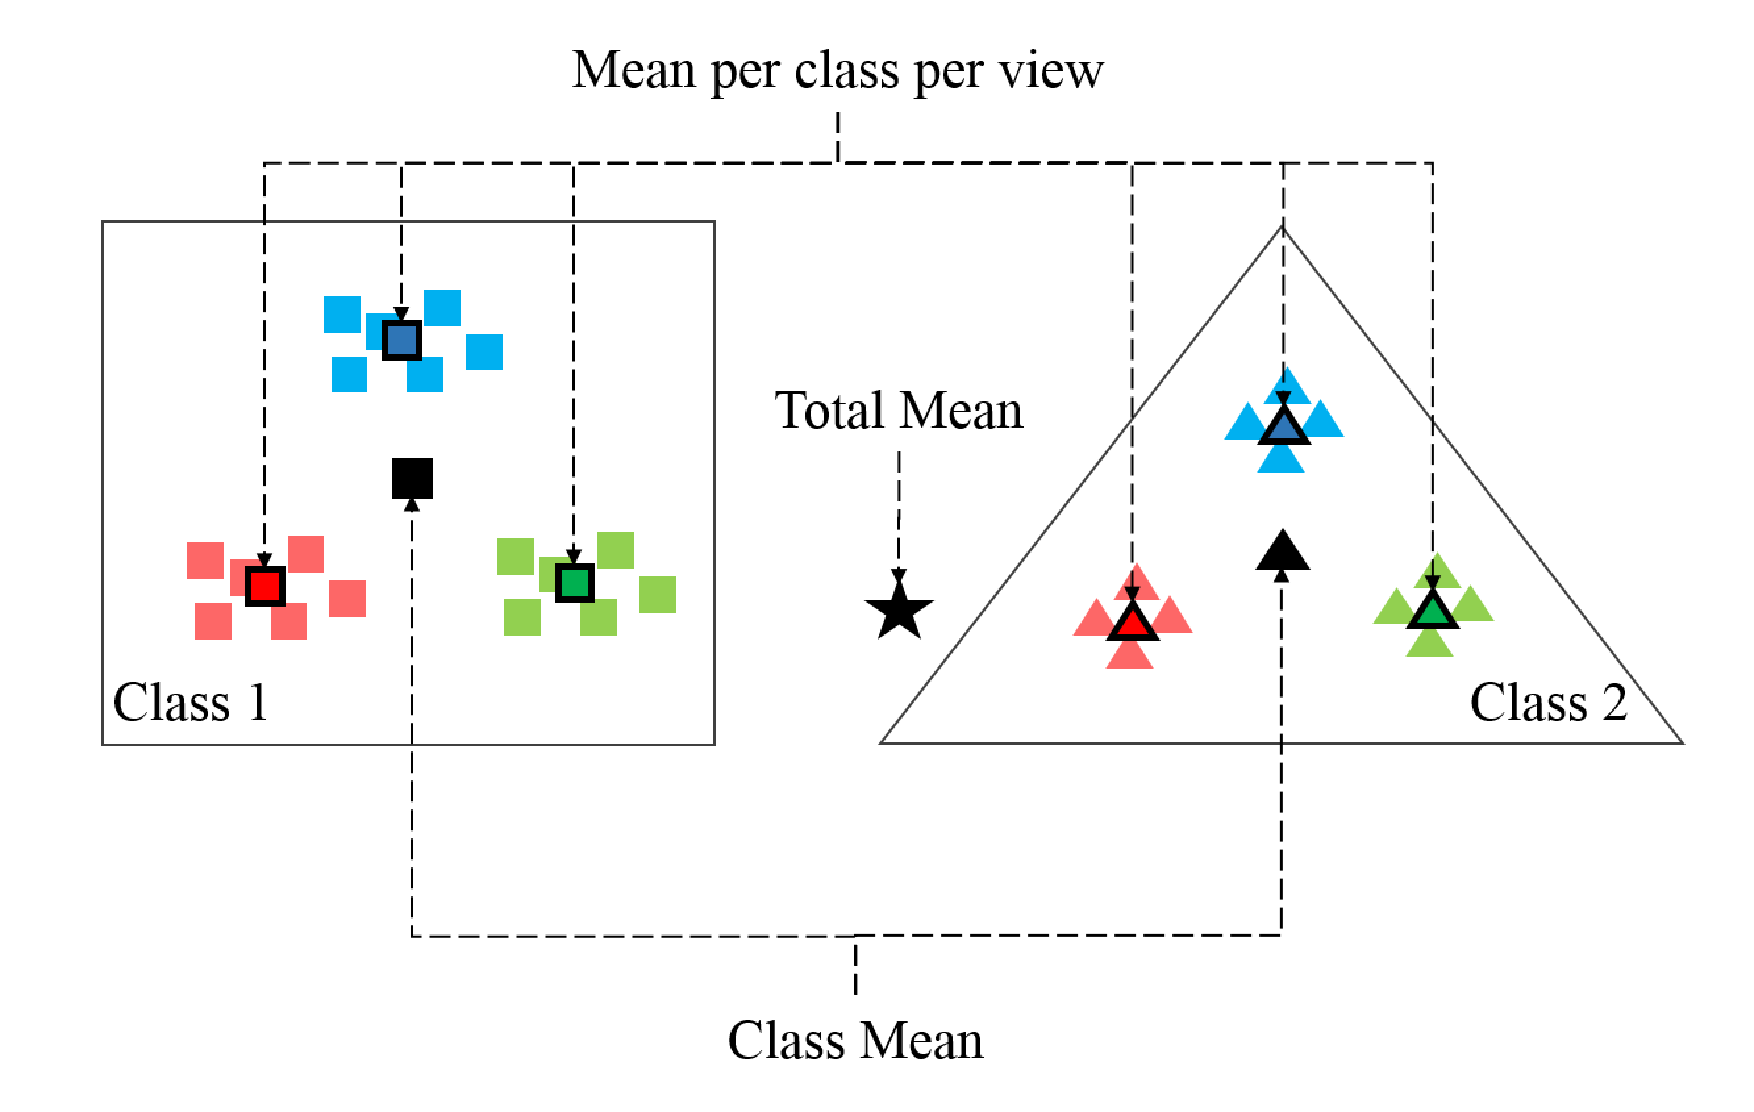
\includegraphics[width=0.85\textwidth]{Figures/Notations/Fig1.pdf}
	\caption{The figure shows the three means pictorially. Three views are shown with three colors- blue, red and green. Two classes, Class1 and Class2, are depicted with squares and triangles, respectively.}
	\label{fig:Means}
\end{figure}


\begin{table}[t]
	\centering
	\caption{Notations and Formulae}
	\label{tab:Equations}
		\begin{tabular}{l l} \toprule
		Notations & Formulae \\
		\midrule
		$n_{ij}$ & - \\[0.2cm] 
		$n_{i}$ & $\sum\limits_{j=1}^{v} n_{ij}$ \\[0.2cm] 
		$n$ & $\sum\limits_{i=1}^{c} n_i$ \\[0.2cm] 
		$\textbf{m}_{ij}^{(\textbf{x})}$ & $ \frac{1}{n_{ij}} \sum\limits_{k=1}^{n_{ij}} \textbf{x}_{ijk}$ \\[0.2cm] 
		$\textbf{m}_i$ & $\frac{1}{n_i} \sum\limits_{j=1}^{v} \sum\limits_{k=1}^{n_{ij}} \textbf{y}_{ijk}$ \\[0.2cm] 
		$\textbf{m}$ & $\frac{1}{n} \sum\limits_{i=1}^{c} \sum\limits_{j=1}^{v} \sum\limits_{k=1}^{n_{ij}} \textbf{y}_{ijk}$ \\
		
		\bottomrule
	\end{tabular}
\end{table}


The increments in the dataset can be of two types: (i) data sample increment- where the number of views remains the same and only the number of data samples changes over time, or (ii) view increment- where the number of data samples remains the same and the number of views changes over time. The increase or decrease in the number of data samples can be sequential (one-by-one) or in chunks (groups of data samples). A set of data samples to be added/deleted is denoted by $\bar{\mathcal{X}}$. If any data sample from $\bar{\mathcal{X}}$ belongs to a new class, this class is denoted by $N$, and if it belongs to an already existing class, we denote its class by $E$. The data sample count or the means related to $\bar{\mathcal{X}}$ are denoted with a bar symbol (e.g., $\bar{m}$) over them and those related to the updated dataset ($\mathcal{X}'$) are denoted with a prime symbol over them (e.g., $m'$).














\section{Assumptions}
\label{sec:Assumptions}
We first state three fundamental assumptions made by all of the four methods.
\begin{itemize}
	\item[A)] The label of the new data sample is made available at the time of its inclusion.
	\item[-] As all the four methods belong to the supervised learning domain, the class label of a data sample is a non-negotiable requirement. As the model is updated as soon as new data is added, without a label, the data sample will be of no use to the algorithm and will be discarded.
	
	\item[B)] Each data sample is present in all of the $v$ views.
	\item[-] This is one of the fundamental assumptions of multi-view learning. All of the views are assumed to contain the information of each data sample in the dataset. In the real world, this may not always be true. Hence, some efforts are being made towards approximating the missing view information \cite{XuTX15, ZhangZZSJ18}.
	
	\item[C)] All of the views agree with each other on the labels of the training data samples.
	\item[-] This is another fundamental assumption of multi-view learning and is very intuitive too. As all the views give information about the same object to solve the same problem, they must agree on the class to which the given sample belongs. If the views disagree on the label, the data sample cannot be used for training, as supervised learning is based on the labeled data.
\end{itemize}

\noindent
Other assumptions made by data sample incremental/decremental methods-
\begin{itemize}
	\item[a)] At the start of the learning process, we may or may not have any existing data samples, i.e., $n \geqslant 0$. 
	\item[-] All of the incremental/decremental methods presented in this thesis support learning from scratch (cold-start) or learning on top of the already existing model (warm-start) without any change in the formulations. Hence, these methods work as well when there is no previous model as they work when updating a previously existing model.
	
	\item[b)] New data samples may belong to an already existing class or a new class.
	\item[-] All of these methods support the addition of new data samples to already existing classes or to a previously unseen class in any increment. MvIDA presents these cases as different specialized formulations. However, both the cases can be taken care of by one generalized formulation as demonstrated with 2DMvIDDA formulations.
	
	\item[c)] In the case of addition, all the views of new data samples are added at once to the dataset.
	\item[-] This assumption is the same as Assumption (B), but written separately in the incremental context because the learning method expects that all the data belonging to a data sample be available at the time of training. So, if one or more views of a new data sample are missing, it cannot be included in the updated model as it violates the fundamental assumption of multi-view learning.
	
	\item[d)] In the case of deletion, all views of the data samples to be deleted are removed from the dataset.
	\item[-] Same as in the case of addition, if we wish to remove a data sample, it has to be removed completely. Information from all the views of a data sample belongs to that data sample. Hence, all of it is removed when deleting that data sample.
	
\end{itemize}

\noindent
Other assumptions made by view incremental/decremental methods-
\begin{itemize}
	\item[a)] At the start of the learning process, one or more views of data samples may have already been presented.
	\item[-] Similar to the first assumption of \textit{data sample increment} above, this assumption states that the learning method is capable of learning a new model when no data was present previously, as well as updating an already existing model.
	
	\item[b)] In the case of addition, new views of all the existing data samples are added at once.
	\item[-] As Assumption-B states, a data sample must be present in all the views. Hence, whenever a new view is added, it must contain the information of all the data samples that exist in the previous views. If any data sample is missing in a new view, the model cannot accept that view for training.
	
	\item[c)] In the case of deletion, the whole view is deleted at once.
	\item[-] Same as above, a view cannot be partially removed as it will violate the fundamental assumption of multi-view learning. If the whole view is deleted, the remaining views still confirm to the assumption that each data sample is present in all the views.
	
\end{itemize}














\section{Datasets}
\label{sec:Dataset}
\hspace{0.8cm}In this section, we first present the details of 1D datasets used for experiments on the 1D methods in chapter \ref{ch:MvIDA} and \ref{ch:VIDMvDA}. We then present the details of 2D datasets used by the 2D methods in chapter \ref{ch:2DMvDA} and \ref{ch:2DMvIDDA}.



\subsection{1D Datasets}
\label{subs:1D_Data}
\hspace{0.8cm}We have used three widely used multi-view datasets for the experiments. All datasets are based on images and their features. Each feature of these images comprises a different view.

\subsubsection{Handwritten Digits Dataset}
\hspace{0.8cm}Handwritten Digits Dataset \cite{BlakeM98Digits} is from the UCI Machine Learning Repository. This dataset contains features extracted from 2000 images of handwritten digits from Dutch utility maps. There are ten classes, one corresponding to each digit from 0 to 9, and each class has 200 images. Each set of features constitutes one view. Details of the description of views and their corresponding dimensions are given in Table \ref{tab:Digits}.

\begin{table}[h]
	\centering
	\caption{Details of Handwritten Digits Dataset}
	\label{tab:Digits}
	\begin{tabular}{c l r} \toprule
		
		\textbf{View\#} & \textbf{Description of View} & \textbf{Dimension} \\ \midrule
		1 & Profile correlations & 216 \\ 
		2 & Fourier coefficients & 76 \\ 
		3 & Karhunen-Love coefficients & 64 \\ 
		4 & Morphological features & 6 \\ 
		5 & Pixel averages in 2 x 3 windows & 240 \\ 
		6 & Zernike moments & 47 \\ \bottomrule
		
	\end{tabular}
\end{table}




\subsubsection{Caltech-7 Dataset}
\hspace{0.8cm}Caltech-7 is a subset of Caltech-101 dataset \cite{FeiFP04Caltech}. This data set contains a total of 1000 images of 7 distinct objects, namely, Faces (435), Motorbikes (324), Dollar-bill (52), Garfield (34), Snoopy (35),  Stop-sign (64), and Windsor-chair (56). Numbers in the brackets denote the cardinality of each class. Each image has a size of around $300 \times 200$ pixels. Six views are composed of six different features extracted from the images. Description of the views and their dimensions are given in Table \ref{tab:Caltech}.

\begin{table}[h]
	\centering
	\caption{Details of Caltech-7 Dataset}
	\label{tab:Caltech}
	\begin{tabular}{c l r} \toprule
		
		\textbf{View\#} & \textbf{Description of View} & \textbf{Dimension} \\ \midrule
		1 & Cenhist Features(CEN) & 254 \\ 
		2 & Gabor Wavelet Features(GAB) & 48 \\ 
		3 & Gist Features(GIS) & 512 \\ 
		4 & Histogram of Oriented Gradients(HOG) & 1984 \\ 
		5 & Local Binary Pattern(LBP) & 928 \\ 
		6 & Wavelet Moments(WAV) & 40 \\ \bottomrule
			
	\end{tabular}
\end{table}




\subsubsection{AwA Dataset}
\hspace{0.8cm}AwA (Animals with Attributes) is a large dataset \cite{LampertNH09} containing a total of 30475 images of 50 animals. The cardinality of each of the 50 classes is different and ranges from 92 to 1168. This dataset has six image features extracted from the original images. Each feature is considered as one view. Description of the views and their dimensions are given in Table \ref{tab:AwA}.

\begin{table}[h]
	\centering
	\caption{Details of AwA Dataset}
	\label{tab:AwA}
	\begin{tabular}{c l r} \toprule
		
		\textbf{View\#} & \textbf{Description of View} & \textbf{Dimension} \\ \midrule
		1 & Color Histogram(CQ) & 2688 \\ 
		2 & Local Self-similarity Features(LSS) & 2000 \\ 
		3 & Pyramid HOG(PHOG) & 252 \\ 
		4 & Scale-Invariant Feature Transform(SIFT) & 2000 \\ 
		5 & Color SIFT(RGBSIFT) & 2000 \\ 
		6 & Speeded-Up Robust Features(SURF) & 2000 \\ \bottomrule
			
	\end{tabular}
\end{table}







\subsection{2D Datasets}
\label{subs:2D_Data}
\hspace{0.8cm}For experiments involving the 2D methods, we have used four widely used multi-view image datasets: the IMPART face dataset \cite{KimEBH18}, the MSSpoof dataset \cite{ChingovskaEAM16}, the Stereo face dataset \cite{FransensSG05} and the ORL dataset \cite{ATnT-ORL}. The first three datasets are based on images of faces taken from different angles. Photographs of the participants taken from one angle compose one view in each of these datasets. As the ORL dataset contains photographs of the participants only from the front view, we have extracted 2D features from these images to make up two more views. Detailed information about all datasets is provided below. Due to the higher memory requirements of 1D methods, we have rescaled the images from original datasets and used them for the experiments that include such methods. However, for experiments that compare only the 2D methods, we have used original datasets to show the full strength of the 2D methods.



\subsubsection{IMPART Face Dataset}
\begin{table}[t]
	\centering
	\caption{Details of IMPART Face Dataset}
	\label{tab:IMPART}
	\begin{tabular}{c l c c} \toprule
		
		\textbf{View\#} & \textbf{Description of View} & \textbf{Dimensions} & \textbf{Rescaled to} \\ \midrule
		1 & Photographs from angle $0^{\circ}$ & $1920 \times 1080$ & $54 \times 96$ \\ 
		2 & Photographs from angle $30^{\circ}$ & $1920 \times 1080$ & $54 \times 96$ \\ 
		3 & Photographs from angle $45^{\circ}$ & $1920 \times 1080$ & $54 \times 96$ \\ 
		4 & Photographs from angle $-30^{\circ}$ & $1920 \times 1080$ & $54 \times 96$ \\ 
		5 & Photographs from angle $-45^{\circ}$ & $1920 \times 1080$ & $54 \times 96$ \\ \bottomrule
		
	\end{tabular}
\end{table}

\hspace{0.8cm}IMPART Face Dataset \cite{KimEBH18} was created within the EU FP7 IMPART project. This dataset contains photographs of 10 participants - seven males and three females. Each person corresponds to one class. Five different views of the participants are captured from five different angles. The description of views and their corresponding dimensions are given in Table \ref{tab:IMPART}. Each view contains six photographs of each participant that correspond to six facial expressions: neutral, anger, fear, happiness, sadness, and surprise.




\subsubsection{MSSpoof Dataset}
\begin{table}[t]
	\centering
	\caption{Details of MSSpoof Dataset}
	\label{tab:MSSpoof}
	\begin{tabular}{c l c c} \toprule
		
		\textbf{View\#} & \textbf{Description of View} & \textbf{Dimensions} & \textbf{Rescaled to} \\ \midrule
		1 & VIS spectrum photographs & $1024 \times 1280$ & $64 \times 80$ \\ 
		2 & NIR spectrum photographs & $1024 \times 1280$ & $64 \times 80$ \\ \bottomrule
			
	\end{tabular}
\end{table}

\hspace{0.8cm}We have taken a subset of the MSSpoof dataset \cite{ChingovskaEAM16}. This subset contains photographs of 15 participants, hence, 15 classes. Out of two views, one contains photographs in the visual spectrum, and the other contains photographs in the infra-red spectrum. The number of photographs per view per person is 28. Description of the views and their dimensions are given in Table \ref{tab:MSSpoof}.








\subsubsection{Stereo Face Dataset}
\hspace{0.8cm}Stereo Face Dataset \cite{FransensSG05} contains photographs of 100 participants (55 males and 45 females). Two cameras are used to provide two views, i.e., the angles of capture. Each camera captures eight photographs per person in different poses. Details of views and their dimensions are given in Table \ref{tab:SF}.


\begin{table}[h]
	\centering
	\caption{Details of Stereo Face Dataset}
	\label{tab:SF}
	\begin{tabular}{c l c c} \toprule
		
		\textbf{View\#} & \textbf{Description of View} & \textbf{Dimensions} & \textbf{Rescaled to} \\ \midrule
		1 & Photographs by Camera-1 & $480 \times 640$ & $96 \times 128$ \\ 
		2 & Photographs by Camera-2 & $480 \times 640$ & $96 \times 128$ \\ \bottomrule
			
	\end{tabular}
\end{table}




\subsubsection{ORL Dataset}
\hspace{0.8cm}ORL \cite{ATnT-ORL} is a face dataset created in 1992 consisting of 400 images. This dataset contains ten photographs of each participant taken from different angles over two years. There are 40 such participants, hence 40 classes. We extracted the FFT \cite{CooleyLW69} and the Canny \cite{Canny86} features from these images and used them as two views along with the original images as the first view. Details of views are given in Table \ref{tab:ORL}.

\begin{table}[h]
	\centering
	\caption{Details of ORL Dataset}
	\label{tab:ORL}
	\begin{tabular}{c l c c} \toprule
		
		\textbf{View\#} & \textbf{Description of View} & \textbf{Dimensions} & \textbf{Rescaled to} \\ \midrule
		1 & Original Images & $112 \times 92$ & $56 \times 46$ \\ 
		2 & FFT & $112 \times 92$ & $56 \times 46$ \\ 
		3 & Canny Features & $112 \times 92$ & $56 \times 46$ \\ \bottomrule
			
	\end{tabular}
\end{table}









\chapterend
\cleardoublepage